\documentclass[conference]{IEEEtran}
\usepackage{amsmath,amssymb}
\usepackage{graphicx}
\usepackage{booktabs}
\usepackage{array}
\usepackage{multirow}
\usepackage{cite}
\usepackage[hidelinks]{hyperref}
\usepackage{balance}

\graphicspath{{figures/}}

\newcommand{\tez}{Tezcat}

\begin{document}

\title{Tezcat: A Deterministic, Provenance-Aware Laboratory for
Experimental Research on Emergent Financial-Market Phenomena}

\author{\IEEEauthorblockN{Satvik Anand}
\IEEEauthorblockA{Registration No.\ RA2311026010278\\
\textit{[Institutional affiliation not established in repository
materials; placeholder retained deliberately]}}}

\maketitle

\begin{abstract}
Financial markets exhibit emergent phenomena---heavy-tailed returns,
volatility clustering, liquidity crises, bubbles, flash crashes, and
deleveraging cascades---whose mechanistic origins are difficult to
isolate from historical data alone, while stylized theoretical models
abstract away the market microstructure through which such phenomena
propagate. We present \tez{}, a deterministic, provenance-aware
experimental laboratory in which researchers construct artificial
markets from heterogeneous trading agents interacting through a genuine
price--time-priority limit order book, perturb individual mechanisms
under controlled conditions, execute replicated experiment designs, and
reproduce every published number from content-addressed identities.
\tez{} contributes a reproducibility architecture (immutable experiment
versions, deterministic seed allocation, canonical serialization,
hash-chained event logs, state and event hashes, artifact-only
reporting, and replay), an operational execution layer with provably
order-independent parallelism, a read-only external event-market
intelligence layer over Kalshi and Polymarket with immutable
checksummed datasets and hypothesis-generating event signatures, and a
bridge that exports deterministic synthetic market worlds into the
NautilusTrader backtesting engine for strategy evaluation under
controlled market ecologies. In a 420-run leverage$\times$liquidity
factorial conducted entirely through the platform's own research
surface, the leverage effect on maximum drawdown was large and
threshold-like ($+0.113$ at the extremes; $0/60$ crashes at a
$2\times$ leverage cap), while the pre-registered
leverage$\times$illiquidity interaction was \emph{rejected}
($+0.015$, 95\% CI $[-0.023, +0.057]$): forced-liquidation volume
concentrated in \emph{deeper} books, indicating that within this model
ecology liquidity acts as a transmission channel for deleveraging
rather than a simple cushion. \tez{} is a simulation laboratory for
mechanism experiments; it does not predict real markets, and no claim
in this paper should be read as a real-market forecast.
\end{abstract}

\begin{IEEEkeywords}
agent-based simulation, market microstructure, limit order book,
reproducibility, provenance, emergent phenomena, leverage, liquidity,
backtesting, prediction markets
\end{IEEEkeywords}

\section{Introduction}
\label{sec:intro}
Financial markets are complex adaptive systems whose most consequential
behaviors---crashes, liquidity evaporation, leverage spirals, regime
shifts---are \emph{emergent}: they arise from interactions among
heterogeneous participants, microstructural rules, and feedback loops
rather than from any single actor's intent
\cite{arthur1997,farmer2009,hommes2006}. Three established
methodological families each illuminate part of this problem while
leaving a gap. Empirical analysis of historical data documents robust
statistical regularities \cite{cont2001} but rarely supports
mechanism-level causal attribution, because the historical record is a
single uncontrolled realization. Stylized theoretical models
\cite{kyle1985,glosten1985} isolate mechanisms analytically but
abstract away the order-book microstructure through which real
disturbances propagate. Machine-learning forecasting systems optimize
predictive accuracy but are structurally unsuited to controlled
mechanism experiments: their objective is extrapolation, not
intervention.

\tez{} occupies a fourth position: \emph{controlled synthetic market
experimentation}. The system provides an artificial market in which
price is endogenous---formed exclusively by order flow through a
price--time-priority central limit order book (CLOB)---populated by
heterogeneous agent classes with adaptive memory, subject to scripted
shocks, margin constraints, and regime-dependent behavior. Around this
engine, \tez{} builds the apparatus of experimental science:
pre-registered designs with control and treatment arms, mandatory
replication, deterministic seed allocation, immutable content-addressed
experiment identities, hash-chained event provenance, statistical
analysis with multiplicity control, artifact-only reporting, and a
\texttt{reproduce} verb that re-executes experiments and verifies every
stored hash. The intent is that a hypothesis about a market mechanism
becomes a falsifiable, replicable, and reproducible experiment---and
that a rejected hypothesis is a first-class result.

Two boundary statements govern everything that follows. First,
\textbf{\tez{} does not predict real markets}; it studies which
mechanisms \emph{can} generate observed classes of phenomena under
explicit assumptions. Second, external market data (Kalshi, Polymarket)
enters only as read-only research observations that inform experiment
design and calibration targets; it never drives the simulation kernel,
and the platform contains no trading, wallet, or order-routing
functionality toward any real venue.

The contributions of this paper are:
\begin{itemize}
\item[\textbf{C1}] a deterministic agent-based market ecology built
around a genuine price--time-priority CLOB with reservation-based
accounting and endogenous price formation (Sec.~\ref{sec:engine});
\item[\textbf{C2}] a reproducibility architecture based on immutable
experiment versions, canonical serialization, deterministic seed
allocation, state/event hashes, hash-chained event logs, artifact
manifests, and replay (Sec.~\ref{sec:repro});
\item[\textbf{C3}] a complete research workflow connecting
specification $\rightarrow$ replication $\rightarrow$ statistical
analysis $\rightarrow$ artifact-only reporting $\rightarrow$
reproduction (Sec.~\ref{sec:workflow});
\item[\textbf{C4}] a custom scenario system that compiles user-defined
market designs into the same canonical experiment machinery
(Sec.~\ref{sec:scenario});
\item[\textbf{C5}] TradeOps, an operational layer providing resumable
batches, worker parallelism with serial-equivalent results, retries,
duplicate-execution guards, and explicit failure semantics
(Sec.~\ref{sec:scenario});
\item[\textbf{C6}] a stylized-facts and calibration layer with enforced
out-of-sample validation and honestly reported identifiability limits
(Sec.~\ref{sec:stylized});
\item[\textbf{C7}] a read-only external event-market intelligence layer
(Kalshi, Polymarket) with immutable checksummed datasets and event
signatures that seed synthetic experiments (Sec.~\ref{sec:external});
\item[\textbf{C8}] a bridge exporting deterministic synthetic market
worlds into NautilusTrader for strategy evaluation under controlled
ecologies (Sec.~\ref{sec:lab});
\item[\textbf{C9}] a container-first deployment architecture, with an
honest classification of which components are implemented versus
planned (Sec.~\ref{sec:devops});
\item[\textbf{C10}] empirical mechanism$\rightarrow$phenomenon
demonstrations, centered on a 420-run leverage$\times$liquidity
factorial whose pre-registered interaction hypothesis was rejected and
which surfaced a non-monotonic liquidity effect
(Sec.~\ref{sec:casestudy}).
\end{itemize}
We claim novelty for the \emph{combination} (Sec.~\ref{sec:gap}), not
for each component individually.

\section{Background and Related Work}
\label{sec:related}

\subsection{Agent-Based Computational Finance}
The Santa Fe artificial stock market \cite{arthur1997} established that
heterogeneous, adaptively learning agents can endogenously generate
market phenomena that representative-agent equilibria cannot. Lux and
Marchesi \cite{lux1999} showed that interaction between chartists and
fundamentalists produces scaling and volatility clustering consistent
with empirical data. Surveys by LeBaron \cite{lebaron2006}, Tesfatsion
\cite{tesfatsion2006}, and Hommes \cite{hommes2006} consolidate this
tradition, and Farmer and Foley \cite{farmer2009} argue for agent-based
modeling as policy-relevant scientific infrastructure. Gode and Sunder
\cite{gode1993} demonstrated that even zero-intelligence traders
interacting through a double auction generate meaningful market-level
regularities---a caution against over-attributing structure to agent
sophistication, which \tez{} inherits by including a noise-trader class.

\subsection{Market Microstructure and Order Books}
Kyle \cite{kyle1985} and Glosten--Milgrom \cite{glosten1985} formalize
price formation under asymmetric information; Bouchaud \emph{et al.}
\cite{bouchaud2002} document the statistical structure of real limit
order books; Cont, Stoikov, and Talreja \cite{cont2010} model order-book
dynamics as a stochastic queueing system; Chiarella and Iori
\cite{chiarella2002} study double-auction microstructure by simulation.
\tez{} adopts the simulation stance with an explicit operational CLOB:
price--time priority, tick snapping, partial fills, order expiry, and
declared self-trade semantics.

\subsection{Stylized Facts}
Cont \cite{cont2001} catalogs the empirical properties any credible
market model should confront: absence of linear return autocorrelation,
heavy tails, volatility clustering, and related regularities. \tez{}'s
feature extractor (Sec.~\ref{sec:stylized}) follows this catalog
directly.

\subsection{Leverage, Liquidity, and Endogenous Instability}
Geanakoplos \cite{geanakoplos2010} develops the leverage cycle; Adrian
and Shin \cite{adrian2010} document procyclical intermediary leverage;
Brunnermeier and Pedersen \cite{brunnermeier2009} model mutually
reinforcing market and funding liquidity spirals; Shleifer and Vishny
\cite{shleifer2011} survey fire-sale dynamics. This literature
motivates \tez{}'s margin engine, in which forced liquidation is
\emph{actual order flow} through the matching engine rather than an
accounting adjustment---a design decision that proved decisive for the
case study of Sec.~\ref{sec:casestudy}.

\subsection{Reproducible Computational Science}
Peng \cite{peng2011} and Sandve \emph{et al.} \cite{sandve2013} argue
that computational claims require executable provenance; Boettiger
\cite{boettiger2015} connects reproducibility to containerization.
\tez{} operationalizes these principles for market simulation:
content-addressed experiment identity, deterministic replay, and
artifact-only reporting are enforced by the system rather than left to
author discipline.

\subsection{Market Simulation and Backtesting Infrastructure}
ABIDES \cite{byrd2020} is the closest system relative: a discrete-event
multi-agent market simulator with realistic exchange messaging. \tez{}
differs in emphasis rather than in kind: its core investment is the
scientific workflow surrounding the simulator (immutable experiment
objects, enforced replication, hash-verified reproduction, artifact-only
reports) and the outward bridges to external event-market observation
and strategy evaluation. NautilusTrader \cite{nautilustrader} is an
event-driven backtesting/trading engine; \tez{} uses it strictly as a
backtest-side consumer of exported synthetic worlds
(Sec.~\ref{sec:lab}).

\subsection{Prediction and Event Markets}
Wolfers and Zitzewitz \cite{wolfers2004} and Arrow \emph{et al.}
\cite{arrow2008} discuss prediction markets as information-aggregation
mechanisms whose prices are informative but not identical to true event
probabilities. \tez{} adopts this exact framing: Kalshi
\cite{kalshiapi} and Polymarket \cite{polymarketapi} observations are
labeled \emph{market-implied probability proxies} throughout the system
(Sec.~\ref{sec:external}).

Table~\ref{tab:gap} positions \tez{} against representative prior work
without diminishing it: each cited line of research is stronger than
\tez{} within its own aims.

\begin{table}[t]
\caption{Literature positioning (representative, not exhaustive)}
\label{tab:gap}
\centering
\scriptsize
\setlength{\tabcolsep}{3pt}
\begin{tabular}{>{\raggedright\arraybackslash}p{1.5cm}>{\raggedright\arraybackslash}p{1.3cm}>{\raggedright\arraybackslash}p{2.05cm}>{\raggedright\arraybackslash}p{2.3cm}}
\toprule
\textbf{Work} & \textbf{Domain} & \textbf{Strength} &
\textbf{Difference from \tez{}} \\
\midrule
Arthur \emph{et al.} \cite{arthur1997}; Lux \& Mar\-che\-si \cite{lux1999} &
agent-based finance & endogenous expectations; emergent scaling &
no CLOB microstructure; no content-addressed reproduction workflow \\
Kyle \cite{kyle1985}; Glosten--Milgrom \cite{glosten1985} &
micro\-structure theory & analytic causal clarity &
abstracted book; not an experimental platform \\
Cont \emph{et al.} \cite{cont2010}; Bouchaud \emph{et al.}
\cite{bouchaud2002} & order-book modeling & empirically grounded book
dynamics & no heterogeneous behavioral ecology or experiment engine \\
ABIDES \cite{byrd2020} & market simulation & high-fidelity exchange
messaging & \tez{} adds immutable experiment identity, hash-verified
reproduction, external-observation and strategy bridges \\
Nautilus\-Trader \cite{nautilustrader} & backtesting engine &
production-grade event-driven execution & consumes historical/synthetic
data; does not generate controlled ecologies \\
Peng \cite{peng2011}; Sandve \emph{et al.} \cite{sandve2013} &
reproduci\-bility & principles and practices & \tez{} enforces them
mechanically for market experiments \\
\bottomrule
\end{tabular}
\end{table}

\section{Research Gap and Design Requirements}
\label{sec:gap}
Existing market simulators typically provide agent behavior, market
dynamics, and visualization. The gap \tez{} addresses is
\emph{system-level}: no single open platform, to our knowledge,
combines (i) operational CLOB microstructure, (ii) a heterogeneous
behavioral ecology with adaptive memory, (iii) deterministic execution
with immutable, content-addressed experiment identity, (iv) hash-chained
event provenance with replay, checkpointing, and forking, (v) enforced
statistical replication and multiplicity-controlled analysis, (vi)
user-constructed scenarios compiling into one canonical execution path,
(vii) read-only external event-market observation with dataset-level
provenance, (viii) exportable synthetic worlds for strategy evaluation
in an external backtesting engine, and (ix) an operational execution
layer with fault-injection-tested storage---under a container-first
deployment model. We claim the \emph{combination} as the contribution;
individually, most components have precedents cited above.

This gap translates into design requirements that recur throughout the
paper: R1, price must be endogenous; R2, identical inputs must yield
byte-identical outputs; R3, every published number must trace to a
persisted artifact; R4, external data must never silently mutate the
simulation kernel; R5, negative results must be as publishable as
positive ones; and R6, the platform must remain runnable if every
optional external integration is removed.

\section{\tez{} System Architecture}
\label{sec:arch}
Fig.~\ref{fig:arch} shows the implemented architecture; Table
\ref{tab:subsystems} inventories the subsystems. A React/Vite terminal
dashboard and a research CLI drive a FastAPI control plane, beneath
which sit the experiment registry, run manager, research API, and
TradeOps queue. The deterministic ecology engine executes a per-step
loop (shocks $\rightarrow$ regime evaluation $\rightarrow$ agent
decisions $\rightarrow$ matching $\rightarrow$ margin/liquidation
$\rightarrow$ snapshot/metrics/event-log append). The research layer
provides batch execution, statistics, stylized facts, calibration,
replay, and hashing. Two outward-facing layers---external event-market
intelligence (Sec.~\ref{sec:external}) and the synthetic-world /
NautilusTrader bridge (Sec.~\ref{sec:lab})---and a research control
plane that links datasets, forecasts, portfolio decisions, worlds,
backtests, and reports into one artifact graph, complete the system.
Dependency direction is strictly \emph{external systems $\rightarrow$
adapters $\rightarrow$ \tez{}}: the simulation kernel imports neither
the market-data adapters, nor NautilusTrader, nor any optional desk
dependency (requirement R6).

\begin{figure*}[t]
\centering
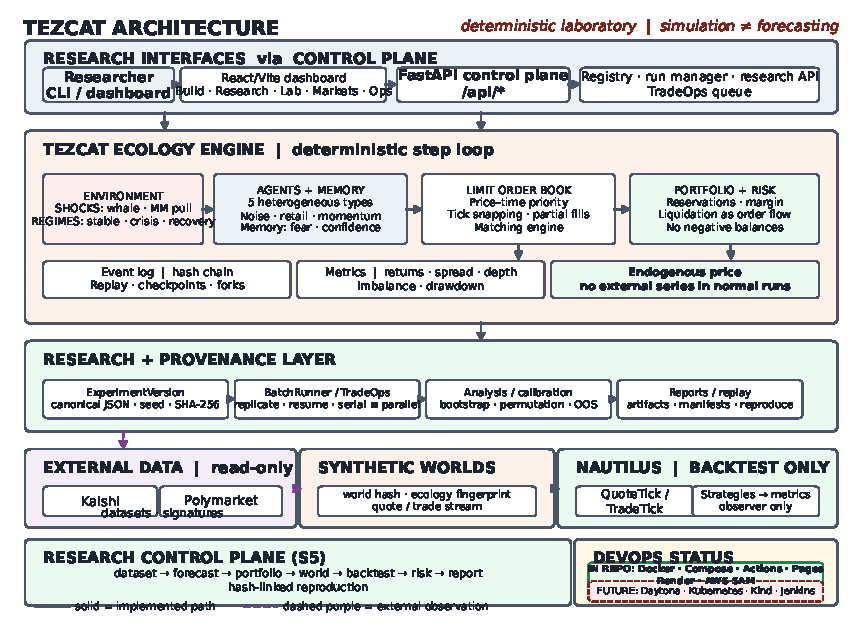
\includegraphics[width=\textwidth]{fig_architecture.pdf}
\caption{Implemented \tez{} architecture. All layers exist in the
audited repository; within the DevOps box, components are explicitly
partitioned into implemented/configured versus future work
(cf.\ Sec.~\ref{sec:devops}).}
\label{fig:arch}
\end{figure*}

\begin{table}[t]
\caption{Subsystem inventory (audited at commit \texttt{af12ef0})}
\label{tab:subsystems}
\centering
\scriptsize
\begin{tabular}{p{2.1cm}p{5.7cm}}
\toprule
\textbf{Subsystem} & \textbf{Role} \\
\midrule
Market engine & CLOB, price--time priority matching, partial fills,
tick snapping, order expiry, declared self-trade policy \\
Agent ecology & five strategy classes with per-agent adaptive memory \\
Shock/regime engines & scripted whale/market-maker/sentiment shocks;
stable/crisis/recovery detection with hysteresis \\
Portfolio/risk & reservation accounting; opt-in margin with
liquidation as real order flow \\
Event log & hash-chained canonical log; replay reconstructs state \\
Registry \& batch & immutable experiment versions; resumable
replicated execution (serial $\equiv$ parallel) \\
Analysis \& reports & bootstrap CIs, permutation tests, Holm
correction; artifact-only rendering \\
Scenario builder \& TradeOps & user scenarios compiled to canonical
experiments; queued, guarded operational execution \\
External intelligence & read-only Kalshi/Polymarket adapters; immutable
datasets; event signatures; research bridge \\
Worlds \& strategy lab & deterministic market worlds; ecology
fingerprints; NautilusTrader backtests \\
Research control plane & typed artifact graph over datasets, forecasts,
portfolio decisions, worlds, backtests, risk, reports \\
\bottomrule
\end{tabular}
\end{table}

\section{Market Ecology Engine}
\label{sec:engine}

\subsection{Formal Setting}
Let $S_t$ denote market state at discrete step $t$, comprising the
order book $B_t$, last price $P_t$, environment variables (sentiment,
regime), and agent states $A_{i,t}$. Each agent draws an action from
its policy conditioned on the public view and its private memory
$m_{i,t}$:
\begin{equation}
a_{i,t} \sim \pi_i\!\left(S_t,\, m_{i,t};\, \theta_i\right),
\end{equation}
where $\theta_i$ are configured behavioral parameters. Submitted
orders $O_t$ transform the book through the matching mechanism
\begin{equation}
B_{t+1} = M\!\left(B_t,\, O_t\right),
\end{equation}
with $M$ implementing price--time priority with partial fills; $P_t$
is the last trade price and is therefore \emph{endogenous}: no external
price series is supplied in normal synthetic experiments (R1). Agent
wealth follows
\begin{equation}
W_{i,t} = C_{i,t} + P_t\, Q_{i,t},
\end{equation}
with cash $C$ and inventory $Q$ governed by reservation accounting:
placing a buy (sell) order reserves cash (inventory), so no agent can
commit resources twice; absent the margin extension, cash and inventory
cannot go negative, and conservation invariants are checked on every
run. Standard observables are computed per step: log return
$r_t = \log(P_t/P_{t-1})$, rolling volatility $\sigma_t$, drawdown
$\mathrm{DD}_t = 1 - P_t/\max_{s\le t}P_s$, spread
$s_t = P^{\mathrm{ask}}_t - P^{\mathrm{bid}}_t$, book depth, order
imbalance $\mathrm{OI}_t$, and an inventory-concentration HHI.

\subsection{Agent Classes and Memory}
Table~\ref{tab:agents} summarizes the five behavioral classes. Each
agent additionally maintains a memory vector $m_{i,t}$ (fear,
confidence, trend belief, value belief) updated from its own
experience; losses raise fear and shrink participation and sizing,
gains do the reverse. Regime state modulates behavior further
(aggression, spread, participation, and cancellation multipliers).

\begin{table}[t]
\caption{Agent classes and behavioral mechanisms}
\label{tab:agents}
\centering
\scriptsize
\begin{tabular}{p{1.5cm}p{6.2cm}}
\toprule
\textbf{Class} & \textbf{Mechanism} \\
\midrule
Noise & seeded random direction/size; liquidity background
(cf.\ zero-intelligence benchmarks \cite{gode1993}) \\
Retail & sentiment- and herding-driven; panic amplification under
crisis regimes \\
Momentum & enters when short-horizon returns exceed a threshold;
trend-following flow \\
Mean reversion & trades deviations from a fundamental anchor within a
band; stabilizing flow \\
Market maker & two-sided quotes around mid with inventory-skewed
pricing; withdraws under stress; primary endogenous liquidity supply \\
\bottomrule
\end{tabular}
\end{table}

\subsection{Shocks, Regimes, Margin}
Shocks are declared, scheduled interventions: whale order programs
(large directional flow sliced over steps), market-maker withdrawal
(quoting suspension), and sentiment shocks (environment shift).
The regime engine classifies stable/crisis/recovery from rolling
drawdown, spread, depth, and volatility with hysteresis (persistence
requirements prevent flapping), and regime events are recorded in the
provenance log. The opt-in margin extension defines equity
$E_{i,t} = C_{i,t} + Q_{i,t} P_t$ and margin ratio
$E_{i,t} / (Q_{i,t} P_t)$; buys are admitted only above an initial
margin $\mathrm{im}$ (leverage cap $\approx 1/\mathrm{im}$), and
maintenance breaches trigger---after a declared delay---a liquidation
\emph{process}: forced market sells in declared slices that pass
through the matching engine like any other flow. Forced volume
therefore measures \emph{fills, not intent}; this distinction is
central to Sec.~\ref{sec:casestudy}. Fig.~\ref{fig:ecology} summarizes
the interaction structure.

\begin{figure}[t]
\centering
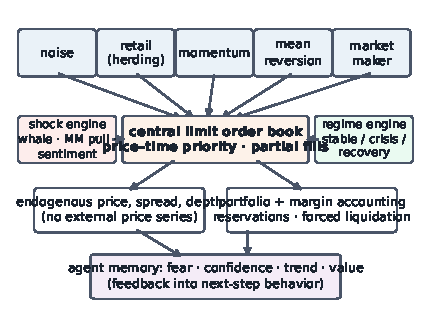
\includegraphics[width=\columnwidth]{fig_ecology.pdf}
\caption{Agent ecology and order-book interaction. Price, spread, and
depth are endogenous outcomes of matched order flow.}
\label{fig:ecology}
\end{figure}

\section{Reproducibility and Scientific Provenance}
\label{sec:repro}

\subsection{Identity}
All configuration is expressed in frozen, schema-versioned models
serialized by a canonical JSON encoder (sorted keys, native types only;
non-canonical values are rejected rather than coerced). An
\emph{ExperimentVersion} binds a base configuration, a validated design
(question, hypothesis, variables, arms/factors, replications, budget),
and a deterministic seed plan into a content-addressed research
identity:
\begin{equation}
H_{\mathrm{exp}} = \mathrm{SHA256}\big(\mathrm{config} \,\|\,
\mathrm{design} \,\|\, \mathrm{seedplan} \,\|\, \mathrm{versions}\big),
\label{eq:hexp}
\end{equation}
where ``versions'' covers the config schema version, seed-allocator
version, and code version. Registered versions are write-once; loading
re-verifies the hash, so schema or code drift fails loudly instead of
silently reinterpreting old records. Per-run seeds derive
deterministically from the root seed, cell name, and replication index,
making them independent of execution order and worker count.

\subsection{Execution Provenance}
Every run appends orders, trades, reservations, shocks, and regime
transitions to a hash-chained event log; the run yields a state hash
(canonical digest of terminal book/portfolio/environment state) and an
event hash (digest over the chained log). Replay rebuilds exact state
from events alone; checkpoints restore bit-identically mid-run, and
forks declare interventions with full parent lineage. Artifacts
(snapshots, trades, metrics, reports) are persisted with manifests, and
reports are rendered \emph{exclusively} from persisted artifacts---a
test verifies that rendered numbers equal independently recomputed
values (R3). Table~\ref{tab:repro} summarizes the guarantees; Fig.\
\ref{fig:repro} shows the pipeline. Later layers extend the same
discipline outward: external datasets, market worlds, strategies, and
research-plane artifacts each carry SHA-256 identities that chain back
to $H_{\mathrm{exp}}$.

\begin{table}[t]
\caption{Reproducibility guarantees (all enforced by tests)}
\label{tab:repro}
\centering
\scriptsize
\begin{tabular}{p{2.6cm}p{5.2cm}}
\toprule
\textbf{Guarantee} & \textbf{Mechanism} \\
\midrule
Same inputs $\Rightarrow$ same run & seeded RNG; deterministic agent
ordering; canonical config \\
Immutable experiment identity & content-addressed
\emph{ExperimentVersion}; write-once registry; hash re-verified on load \\
Order/worker independence & per-run seeds derived from (root, cell,
replication); serial $\equiv$ parallel byte-for-byte \\
Event provenance & hash-chained log; replay reconstructs state;
checkpoint/fork lineage \\
Artifact-backed reporting & reports render only from persisted
artifacts; equality test vs.\ recomputation \\
Chain reproduction & \texttt{tezcat reproduce} re-executes sampled runs
and verifies seeds, state/event hashes, log chains, metrics \\
External/world/strategy identity & dataset hashes, world hashes,
strategy hashes, environment records; version mismatch fails
reproduction \\
\bottomrule
\end{tabular}
\end{table}

\begin{figure}[t]
\centering
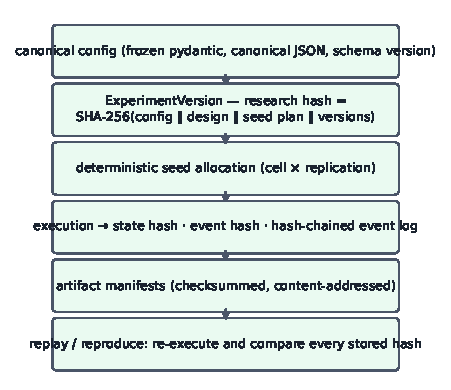
\includegraphics[width=0.94\columnwidth]{fig_repro_pipeline.pdf}
\caption{Provenance pipeline from canonical configuration to
hash-verified reproduction.}
\label{fig:repro}
\end{figure}

\subsection{The Frozen Baseline as Evidence}
Development proceeded in audited phases. Phase F0 froze a seed-42
baseline of the three preset ecologies (51 passing tests) and recorded
their outputs verbatim; every subsequent phase---semantics hardening
(F1), identity/provenance (F2), events/replay, research objects,
batches, analysis, microstructure, risk, stylized facts and calibration
(F9), the research CLI/API/dashboard loop (F10), and parallel
execution with fault injection and differential validation (F11)---was
required to keep that baseline byte-identical. The suite grew from 51
tests (F0) to 208 at the end of S1, then 231 (S2, scenarios and
TradeOps), 335 (S3, external intelligence), 376 (S4, market worlds and
the NautilusTrader bridge), and 415 at the prior paper-audit commit
(\texttt{16448b4}). In the current checkout (\texttt{af12ef0}), the
restored documented offline data provider yields 380 passing tests and
7 explicit skips; the seed-42 determinism gate still reports identical
outputs. A stronger
demonstration appears in Sec.~\ref{sec:casestudy}: an experiment
specification committed several development phases earlier re-minted
its original research hash exactly when re-registered at the audited
commit.

\section{Experiment Design and Research Workflow}
\label{sec:workflow}
A design declares its type (baseline, A/B, ablation, sweep, or
factorial), question, hypothesis, variables, primary metric, arms or
factors, and replications; non-baseline designs \emph{require} at least
two replications (``one seed is a demonstration, not evidence''), and
budgets cap planned runs with explicit, never silent, truncation. The
batch runner executes the design matrix resumably and idempotently;
analysis provides seeded bootstrap confidence intervals, permutation
tests with Holm correction, effect sizes, and $2{\times}2$ interaction
contrasts; reports are artifact-only; and reproduction re-executes
sampled runs against every stored hash. The complete loop is exposed
identically through the CLI
(\texttt{run} / \texttt{analyze} / \texttt{report} /
\texttt{reproduce} / \texttt{list}), the research API, and the
dashboard (Fig.~\ref{fig:workflow}).

\begin{figure}[t]
\centering
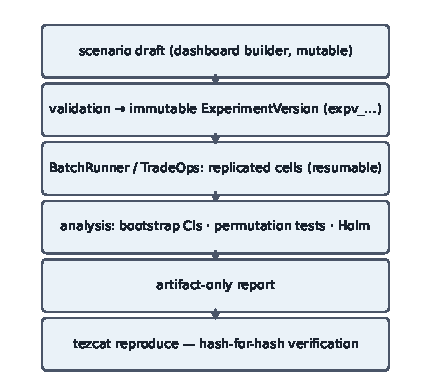
\includegraphics[width=0.94\columnwidth]{fig_workflow.pdf}
\caption{Scenario-to-reproduction workflow. User scenarios compile into
the same immutable experiment machinery used by presets and code-level
specifications (one canonical execution path).}
\label{fig:workflow}
\end{figure}

\section{Custom Scenario Builder and TradeOps}
\label{sec:scenario}

\subsection{Scenario Builder}
The dashboard scenario builder turns preset demonstrations into
user-defined research: market configuration (tick, order-size and age
limits), agent population and behavioral parameters, risk/margin
parameters, shock timeline, and simulation length are edited as a
mutable draft, validated by a dry run through the real
\emph{ExperimentVersion} constructor (surfacing the exact research
identity the design would mint), and then registered immutably.
Scenarios are \emph{not} a second simulation path: no frontend
simulation logic exists, and a compiled scenario is indistinguishable
from a hand-written specification (C4).

\subsection{TradeOps}
TradeOps wraps batch execution in an operational state machine
(\textsc{queued} $\rightarrow$ \textsc{running} $\rightarrow$
\textsc{completed}/\textsc{failed}/\textsc{cancelled}) with worker
processes, capacity guardrails, cooperative cancellation,
identity-preserving retries, a duplicate-execution guard, and persisted
partial results, so an interrupted batch resumes honestly rather than
silently restarting. Parallel execution is required to be
\emph{byte-identical} to serial execution for any worker count; this
property is tested, not assumed. Fault-injection testing of the storage
layer (F11) surfaced a genuine concurrency defect: atomic writes used a
\emph{shared} temporary filename per key, so two writers racing on the
same key collided---one rename won and the other's temporary file
vanished. The fix (writer-unique temporary names incorporating process
and thread identity) is now load-bearing across the registry, world,
dataset, and artifact stores; we report the bug because it illustrates
why fault injection belongs in scientific-infrastructure test suites.

\section{External Event-Market Intelligence}
\label{sec:external}

\subsection{Read-Only Providers, Canonical Semantics}
The S3 layer integrates Kalshi \cite{kalshiapi} and Polymarket
\cite{polymarketapi} as \emph{read-only observation sources}---not
trading integrations: there is no order placement, account, wallet, or
key functionality anywhere in the layer, and public market-data
endpoints are used without credentials. Prediction-market semantics are
preserved by a canonical schema (Event $\rightarrow$ Market
$\rightarrow$ Outcome $\rightarrow$ Observation) in which a YES price
is always a \emph{market-implied probability proxy}
\cite{wolfers2004,arrow2008}, never a forecast or a true probability;
provider-native units (Kalshi cent/dollar representations, Polymarket
decimal strings) are preserved verbatim beside every canonical value,
and each conversion names its rule. The Kalshi adapter covers events,
markets, order books (YES/NO bid representation with the exact binary
identity $\mathrm{ask} = 1 - p^{\mathrm{NO,bid}}$ recorded as the
transform), trades, and candlestick history; the Polymarket adapter
covers the Gamma (metadata), CLOB (books/prices), and Data API (trades)
surfaces. Both adapters implement pagination, token-bucket rate
limiting, retry with backoff, and strict schema-drift detection: a
missing or renamed provider field raises a named error rather than
being silently reinterpreted.

\subsection{Immutable Datasets and Provenance}
Every import follows raw response $\rightarrow$ immutable raw artifact
$\rightarrow$ canonical normalization $\rightarrow$ registered dataset
with SHA-256 checksums of both raw and normalized artifacts, adapter
and schema versions, retrieval provenance, sampling declaration, and
mandatory license/terms metadata with a permitted-use category
(endpoint accessibility is never treated as redistribution
permission). Datasets are content-addressed and write-once; quality
violations (duplicates, timestamp regressions, out-of-range
probabilities) reject a dataset rather than silently cleaning it. The
test suite operates fully offline over labeled synthetic fixtures; no
recorded provider data is bundled.

\subsection{From Observation to Experiment}
The research bridge (Fig.~\ref{fig:s3}) turns an observed episode into
a controlled experiment: a versioned, hashed \emph{event signature}
(pre/post implied probability, $\Delta p$, peak, time-to-peak,
spread/volume/depth changes, and bounded-probability stylized features
computed on $\Delta p$; a logit transform is available but refuses
boundary values rather than clipping) is extracted over a declared
window; rule-based templates propose \emph{candidate mechanisms}
(information shock, herding, momentum amplification, market-maker
withdrawal, thin liquidity) phrased as hypotheses; and an ordinary
\emph{ExperimentVersion} is compiled whose research hash embeds the
dataset identity, so reproduction verifies the experiment \emph{with
respect to that exact dataset version}. Cross-provider analysis is
deliberately conservative: algorithmic event matching caps at
``likely equivalent'' (only human review with recorded rationale can
assert exact equivalence), price differences are labeled
\emph{cross-provider probability divergence} rather than arbitrage,
and lead/lag measurements are labeled observational with no causal
claim.

\begin{figure}[t]
\centering
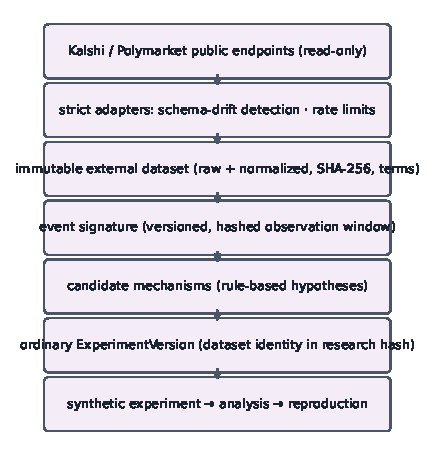
\includegraphics[width=0.94\columnwidth]{fig_s3_pipeline.pdf}
\caption{External event-market intelligence: read-only observation to
reproducible synthetic experiment. External data informs design and
calibration targets; it never mutates the simulation kernel (R4).}
\label{fig:s3}
\end{figure}

\section{Synthetic Market Worlds and the NautilusTrader Bridge}
\label{sec:lab}
A \emph{market world} is one deterministic realization of a registered
experiment cell: (version, cell, replication) fixes the seed, the
engine runs, and the result is captured as a canonical stream---L1
quotes with aggregate side depth as sizes (steps with an empty side are
counted, never fabricated), trades with an honest
\textsc{no\_aggressor} marker (the matcher does not record taker side),
and regime/shock annotations with derived intervals---under a
deterministic step-to-nanosecond time mapping. The world hash covers
the research hash, seed, config/state/event hashes, stream checksums,
time mapping, and a versioned \emph{ecology fingerprint}: a purely
numeric environment identity (relative spread, depth quantiles,
imbalance, return volatility, Hill tail index, volatility clustering,
drawdown/crash flag, trade intensity, regime occupancy, agent
composition). Strategy results thus reference an \emph{environment
identity}, not a data file.

Worlds export to NautilusTrader's \cite{nautilustrader} standard
\texttt{QuoteTick}/\texttt{TradeTick} types after strict validation
(crossed quotes, non-monotone timestamps, and invalid quantities are
rejected), and a hashed reference strategy library (buy-and-hold, EMA
crossover, mean reversion) runs in its backtest engine. All metrics
derive from primary records (the strategy's own submission/fill log
plus the world's quote stream): PnL, drawdown, turnover, fill rate,
slippage versus prevailing mid, exposure, and \emph{regime-conditioned}
breakdowns using \tez{}'s own exported regime intervals. Result
identity is the chain research hash $\rightarrow$ world hash
$\rightarrow$ strategy hash $\rightarrow$ backtest configuration, plus
a recorded environment; reproduction rebuilds the world (hash must
match), re-runs the backtest, and requires byte-identical metrics---a
NautilusTrader version mismatch is reported as \emph{non-identical}
and fails, never silently accepted (Fig.~\ref{fig:s4}).

Two boundaries are explicit. First, the bridge is
\textbf{backtest-only}: no sandbox or live-trading surface exists.
Second, the strategy is an \textbf{observer}: its orders fill against
the exported stream inside NautilusTrader and \emph{do not feed back}
into the \tez{} ecology; market-impact claims are out of scope by
construction, and closing this loop is future work gated on an
explicit co-simulation contract (Sec.~\ref{sec:future}). A further
layer (the S5 research control plane) links datasets, distributional
forecasts from a reference model, cost-aware portfolio sizing
(reference CVaR grid or an optional skfolio adapter \cite{skfolio}),
worlds, backtests, and risk reports into a single typed artifact graph
with whole-chain hash reproduction; we note it for completeness and
audit it in Sec.~\ref{sec:eval}.

\begin{figure}[t]
\centering
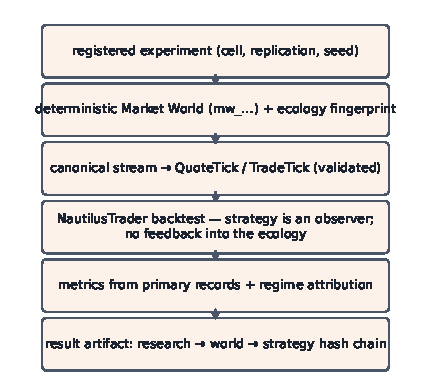
\includegraphics[width=0.94\columnwidth]{fig_s4_bridge.pdf}
\caption{Market-world export and strategy evaluation. The strategy
observes the world; feedback into the ecology is deliberately absent
in the current implementation.}
\label{fig:s4}
\end{figure}

\section{Stylized Facts and Calibration}
\label{sec:stylized}
The feature extractor follows Cont \cite{cont2001}:
return moments, excess kurtosis, Hill tail index, return and
absolute-return autocorrelations at fixed lags, a volatility-clustering
summary, maximum drawdown, and optional volume clustering
(Table~\ref{tab:facts}). Comparison is \emph{ensemble-based}: the
synthetic side is a $\ge$10-replication ensemble, and each target
feature is reported with the ensemble q05--q95 band, an inside/outside
verdict, and a $z$-distance; a partial match is the expected and
informative outcome, not a failure. Calibration is disciplined by
construction: calibration and validation sources must differ (identical
sources are a schema violation), search is a deterministic, budgeted
grid with full evaluation logging and explicit truncation flags,
results are frozen, and validation never re-tunes. Two methodological
findings are reported rather than hidden. First, a pure $|z|$ objective
was evaluated and \emph{rejected} because dividing by ensemble spread
rewards diffuse models; the objective is relative error of the ensemble
mean, with $z$ retained as a diagnostic. Second, identifiability is
real and uneven: tick size (a strong, monotone driver of return
volatility) was recovered exactly from a single target series, whereas
agent \emph{count} proved weakly identifiable---its effect saturates
below single-series noise. Calibration claims are therefore bounded by
what the data can actually identify.

\begin{table}[t]
\caption{Stylized-fact features extracted per series}
\label{tab:facts}
\centering
\scriptsize
\begin{tabular}{p{2.6cm}p{5.2cm}}
\toprule
\textbf{Feature} & \textbf{Definition (implementation-aligned)} \\
\midrule
Return moments & mean, std of $r_t=\log(P_t/P_{t-1})$; skewness \\
Heavy tails & excess kurtosis; Hill tail index over top-decile
$|r_t|$ \\
Linear autocorrelation & $\mathrm{acf}(r_t,\ell)$,
$\ell\in\{1,2,5,10\}$ \\
Volatility clustering & mean $\mathrm{acf}(|r_t|,\ell)$ over the same
lags \\
Drawdown & $\max_t \mathrm{DD}_t$ \\
Activity & volume autocorrelation (when volumes exist) \\
\bottomrule
\end{tabular}
\end{table}

\section{DevOps and Deployment Architecture}
\label{sec:devops}
\tez{} is container-first and locally deployable; Table
\ref{tab:devops} classifies every component by \emph{in-repository
evidence}, per the audit requirement that architecture aspirations must
not be reported as experimental claims. Implemented/configured: a
Dockerfile packaging backend, CLI, and built frontend; Docker Compose
for one-command local orchestration; GitHub Actions workflows for CI
and GitHub Pages deployment of the dashboard; a Render blueprint
deploying the public backend demo with explicit public-demo guardrails;
and an AWS SAM template for optional serverless deployment.
Documented/demonstrated: Daytona-based containerized development
environments (this paper itself was produced in one) and the public
demo runbook. \textbf{No Kubernetes manifests, Minikube/Kind
configuration, or Jenkins pipelines exist in the repository}; these are
future work, and Fig.~\ref{fig:devops} renders that distinction
visually. Containerization also serves reproducibility
\cite{boettiger2015}: environment identity (Python, package, and
adapter versions) is recorded on research artifacts and checked during
reproduction.

\begin{table}[t]
\caption{DevOps components by in-repository evidence}
\label{tab:devops}
\centering
\scriptsize
\begin{tabular}{p{2.2cm}p{2.2cm}p{3.1cm}}
\toprule
\textbf{Component} & \textbf{Status} & \textbf{Evidence} \\
\midrule
Docker & implemented & \texttt{Dockerfile} \\
Docker Compose & implemented & \texttt{docker-compose.yml} \\
GitHub Actions & implemented & workflows \texttt{ci.yml},
\texttt{deploy-pages.yml} \\
GitHub Pages & implemented & Pages deploy workflow; public-demo docs \\
Render & configured & \texttt{render.yaml} blueprint; deployment docs \\
AWS (SAM) & configured & \texttt{infra/templates/}\allowbreak\texttt{template.yaml} \\
Daytona & documented/ demonstrated & \texttt{docs/docker.md};
development environment \\
Kubernetes, Minikube/Kind & future work & no manifests in repository \\
Jenkins & future work & no pipeline in repository \\
\bottomrule
\end{tabular}
\end{table}

\begin{figure}[t]
\centering
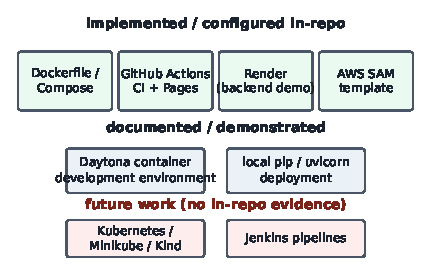
\includegraphics[width=0.9\columnwidth]{fig_devops.pdf}
\caption{Deployment components partitioned by in-repository evidence.}
\label{fig:devops}
\end{figure}

\subsection{Security and Data Governance}
External access is read-only public market data; no credential is
required, stored, or forwarded for any endpoint the adapters use, and
any future credentialed integration is confined to server-side
environment variables (never experiment JSON, hashes, artifacts, logs,
or the frontend). Rate limits are respected by construction; live
provider access is disabled by default (offline fixtures only) and
gated by an explicit server-side opt-in; public-demo mode additionally
restricts imports and caps run sizes. Dataset provenance records
license/terms and permitted use. There is no wallet functionality, no
live trading, and no financial execution of any kind: \tez{} is a
research laboratory, not an execution venue, and its documentation
enumerates claims it must never make (e.g., ``automated hedge fund,''
``predicts crashes'').

\section{Experimental Evaluation}
\label{sec:eval}
All evidence in this section was re-verified at commit
\texttt{af12ef0}; no number is carried forward from documentation
without re-execution unless explicitly labeled as an archived value.

\subsubsection*{A. Determinism} The engine-level gate (same seed
$\Rightarrow$ identical outputs; different seed $\Rightarrow$
different outputs) passes at the audited commit, and the frozen
seed-42 preset baselines (Table~\ref{tab:presets}) remain byte-identical
to their F0 records.

\subsubsection*{B. Reproduction} \texttt{tezcat reproduce} re-executed
sampled runs of the case-study experiments and verified seeds, state
hashes, event hashes, event-log chains, and metrics; the
strategy-bridge and research-plane reproducers additionally verified
world hashes and full artifact-chain hashes, including byte-level
metric equality.

\subsubsection*{C. Parallel equivalence} The 300-run factorial of
Sec.~\ref{sec:casestudy} was re-executed with four worker processes;
because seeds derive from (root, cell, replication), results are
independent of scheduling, and the suite's differential tests assert
serial/parallel byte equality.

\subsubsection*{D. Fault tolerance} Fault-injection tests cover torn
tmp files, crashed writers, duplicate concurrent runners, and provider
failures (timeouts, malformed payloads, schema drift, rate limits);
the shared-tmp-filename defect found by these tests
(Sec.~\ref{sec:scenario}) is fixed and regression-tested.

\subsubsection*{E. Differential validation} An independent reference
matcher is compared against the production matching engine on
generated order streams, guarding the microstructure semantics that
all higher layers depend on.

\subsubsection*{F. Stylized facts} Fig.~\ref{fig:stylized} compares a
12-replication stable-ecology ensemble against the seed-42 flash-crash
series (a synthetic target; no licensed real-market data is bundled).
As expected, tail and clustering features of the crash series fall
outside the stable ensemble's q05--q95 bands while location features
overlap---exactly the discriminating behavior the comparison layer is
designed to expose.

\subsubsection*{G. Calibration} The identifiability results of
Sec.~\ref{sec:stylized} (tick size recovered; agent count weakly
identifiable; $|z|$ objective rejected) are enforced by tests and
documented as methodological findings.

\subsubsection*{H. Strategy evaluation} Sec.~\ref{sec:lab}'s bridge
runs the reference strategies against deterministic worlds with full
provenance; Fig.~\ref{fig:regime} and Table~\ref{tab:strategy} report
a regime-conditioned example, and reproduction requires byte-identical
metrics under a matching NautilusTrader version.

\subsubsection*{I. External integration} The S3 layer's adapter,
normalization, lineage, quality-rejection, matching, and
bridge-to-experiment paths are covered by offline fixture tests,
including an end-to-end flow from fixture import to hash-verified
reproduction of a signature-derived experiment.

\subsubsection*{J. Scenario execution} S2 tests compile dashboard
scenarios into registered experiments and execute them through
TradeOps, confirming the single-execution-path property.

The current suite run comprises \textbf{380 passing tests and 7
skips} at the audited commit (approximately 28\,s wall time in the
development container), spanning unit, property, determinism, replay,
differential, fault-injection, and integration levels. The historical
415-test count belongs to the prior paper-audit commit and is not used
as the current total.

\begin{table}[t]
\caption{Frozen seed-42 preset baselines (F0 audit record, verbatim;
re-verified at the audited commit)}
\label{tab:presets}
\centering
\scriptsize
\setlength{\tabcolsep}{3.5pt}
\begin{tabular}{lrrrr}
\toprule
\textbf{Preset} & \textbf{Steps} & \textbf{Return} &
\textbf{Max DD} & \textbf{Regimes (\% steps)} \\
\midrule
stable\_baseline & 1{,}500 & $-0.05\%$ & $0.10\%$ & stable 100 \\
flash\_crash & 2{,}000 & $+1.85\%$ & $29.39\%$ &
58.3\,/\,15.8\,/\,26.0 (st/cr/rec) \\
bubble\_formation & 2{,}200 & $+15.45\%$ & $17.04\%$ & stable 100 \\
\bottomrule
\end{tabular}
\end{table}

\subsection{Preset Demonstrations}
The three presets are demonstrations, not evidence (single seed). The
flash-crash ecology (whale sell program, market-maker withdrawal, panic
sentiment) produces the canonical anatomy in
Fig.~\ref{fig:anatomy}---price collapse with spread expansion and depth
evaporation, crisis-regime detection, and recovery---while the
momentum-heavy bubble ecology drifts $+15.45\%$
(Fig.~\ref{fig:presets}). The F0 audit records an instructive
definitional honesty case: the bubble run's ``crash'' flag is true
purely because its $17.04\%$ drawdown exceeds a $15\%$ threshold while
the regime engine remains stable throughout---the flag is a drawdown
threshold, not a validated crash event. Fig.~\ref{fig:pnl} shows
aggregate PnL by agent class for the flash-crash run; the whale's
scripted selling transfers wealth into the surviving classes, with
market makers bearing inventory losses (values are from the run report
artifact; single-seed, illustrative only).

\begin{figure}[t]
\centering
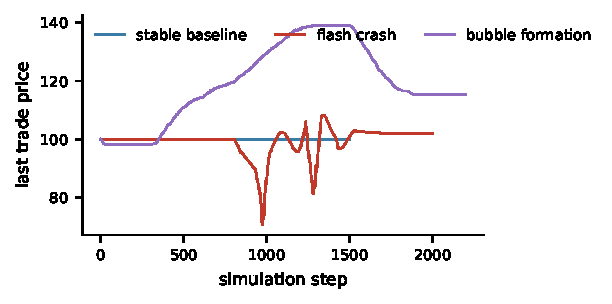
\includegraphics[width=\columnwidth]{fig_presets.pdf}
\caption{Seed-42 price trajectories of the three preset ecologies
(endogenous prices; single-seed demonstrations).}
\label{fig:presets}
\end{figure}

\begin{figure}[t]
\centering
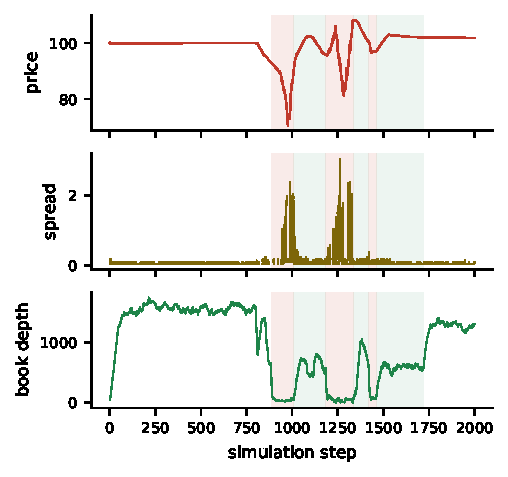
\includegraphics[width=\columnwidth]{fig_flash_anatomy.pdf}
\caption{Flash-crash anatomy (seed 42): last price, quoted spread, and
total book depth; shaded bands mark detected crisis (red) and recovery
(green) regimes.}
\label{fig:anatomy}
\end{figure}

\begin{figure}[t]
\centering
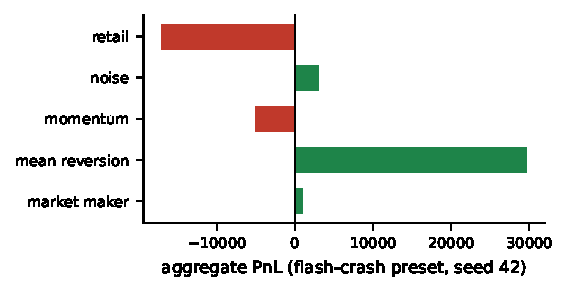
\includegraphics[width=\columnwidth]{fig_agent_pnl.pdf}
\caption{Aggregate PnL by agent class, flash-crash preset (seed 42;
from the persisted run report).}
\label{fig:pnl}
\end{figure}

\begin{figure}[t]
\centering
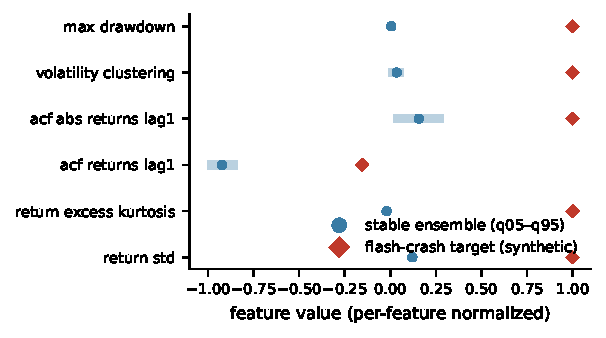
\includegraphics[width=\columnwidth]{fig_stylized.pdf}
\caption{Stylized-facts comparison: stable-ecology ensemble bands
(q05--q95, $n{=}12$) versus the seed-42 flash-crash series as a
synthetic target. Per-feature normalization for display; underlying
values from the feature extractor.}
\label{fig:stylized}
\end{figure}

\subsection{Margin-Spiral A/B (F8)}
The committed specification \texttt{margin\_spiral\_ab.json} asks
whether the leverage cap determines if a pump-and-dump ends in a
liquidation spiral (20 replications per arm, identical shocks and
ecology). Re-executed at the audited commit, it re-minted its original
research identity (\texttt{expv\_417305c181af}) and reproduced the
archived statistics exactly: tight margin ($2\times$ cap) mean max
drawdown $0.0217$ (q95 $0.0306$); loose margin ($10\times$ cap) mean
$0.1847$ (q95 $0.4122$); difference $\Delta = 0.163$, 95\% CI
$[0.103, 0.229]$, Holm-adjusted $p = 0.0005$. Within the synthetic
ecology, leverage is an endogenous mechanism producing a
liquidation-spiral phenomenology---consistent with, but not evidence
about, real-market leverage dynamics
\cite{geanakoplos2010,brunnermeier2009,adrian2010}.

\section{Case Study: Leverage $\times$ Liquidity}
\label{sec:casestudy}
The centerpiece experiment was conducted \emph{as a user} of the
platform, entirely through the public CLI surface, with the hypothesis
pre-stated in the committed study document.

\subsection{Design}
\emph{Question:} does increasing leverage amplify the destabilizing
effect of declining market liquidity? \emph{Pre-stated hypothesis:}
drawdown, forced liquidation, and crash frequency rise with leverage,
and rise \emph{faster} when market-maker liquidity is thin (a positive
leverage$\times$illiquidity interaction). Two committed specifications
over the pump-then-dump margin ecology: a $5{\times}3$ factorial map
(leverage cap $\{2,4,6,8,10\}\times$ via initial margin, market-maker
count $\{1,3,5\}$, 20 replications per cell, 300 runs) and a
$2{\times}2$ extremes design ($\{2\times,10\times\} \times \{1,5\}$
market makers, 30 replications per cell, 120 runs)---420 runs total.
Primary metric: maximum drawdown; secondary: crash frequency (fraction
of seeds with \texttt{crash\_detected}), forced-liquidation volume,
realized volatility.

\subsection{Results}
Both experiments re-minted their archived research identities at the
audited commit (\texttt{expv\_60fabaa6f7ca},
\texttt{expv\_cfc17774801a}; the map's full research hash begins
\texttt{60fabaa6f7ca8453}$\ldots$), and the statistics below are from
that re-execution.

\subsubsection{Leverage: confirmed, threshold-like}
Pooled over liquidity, mean maximum drawdown rises from $0.022$ at
$2\times$ to $0.063$ at $4\times$ and $0.132$--$0.148$ at
$6$--$10\times$; crash frequency is \textbf{0/60 at $2\times$} across
all liquidity levels, rising to 20--65\% per cell at $8$--$10\times$
(Fig.~\ref{fig:heatmap}, Fig.~\ref{fig:levdd},
Table~\ref{tab:levliq}). The $2{\times}2$ main effect of leverage is
$+0.113$ maximum drawdown, replicating and extending the F8 result.

\subsubsection{The pre-registered interaction: rejected}
At the extremes, the leverage$\times$illiquidity interaction contrast
is
\begin{equation*}
+0.0146,\quad 95\%\ \mathrm{CI}\ [-0.0233,\ +0.0567],
\end{equation*}
spanning zero, and the liquidity main effect is $+0.004$---essentially
nothing. Thin liquidity does \emph{not} measurably amplify
leverage-driven drawdowns in this model; the hypothesis is rejected as
stated. We regard this rejection, produced and reproduced by the
platform's own machinery, as a demonstration that the system supports
falsification rather than confirmation.

\subsubsection{The surprise: liquidity as transmission channel}
Forced-liquidation volume concentrates in the \emph{deeper} books
(Table~\ref{tab:levliq}): thin books exhaust, forced sells fail to
fill, and the cascade self-limits; deeper books let deleveraging
actually transact, transmitting price impact into other levered
agents' collateral. The worst observed cell is $8\times$ leverage with
\emph{medium} liquidity (3 market makers): 65\% crash frequency and
the largest mean forced volume (10.5). Because forced volume measures
\emph{fills, not intent} (Sec.~\ref{sec:engine}), this mechanism is
directly readable from the artifacts. \textbf{Within the \tez{}
ecology and this experimental configuration}, market-maker liquidity
under high leverage behaves as a transmission channel for deleveraging
rather than simply a stabilizing cushion---an interaction structure
reminiscent of, but not evidence for, liquidity-spiral accounts of
real markets \cite{brunnermeier2009,shleifer2011}.

\subsubsection{Design lessons}
The effect is non-monotone in liquidity at high leverage, which the
$2{\times}2$ extremes design is structurally unable to detect---the
medium-liquidity spike lives exactly where extremes-only designs do
not look. Crash-frequency cells use $n{=}20$, so the 65\% vs.\ 20\%
contrast carries wide binomial uncertainty; the archived study
explicitly marks the $8\times$/3-MM spike as suggestive and calls for
a higher-$n$ replication of that row. Both caveats are as much results
about experimental design as about the model.

\begin{table}[t]
\caption{Leverage $\times$ liquidity map (re-executed at the audited
commit; $n{=}20$ per cell): mean max drawdown / crash frequency /
mean forced volume filled}
\label{tab:levliq}
\centering
\scriptsize
\begin{tabular}{lccc}
\toprule
\textbf{Leverage} & \textbf{1 MM} & \textbf{3 MM} & \textbf{5 MM} \\
\midrule
$2\times$ & .025 / 0\% / 0 & .020 / 0\% / 0 & .021 / 0\% / 0 \\
$4\times$ & .083 / 15\% / 0 & .064 / 10\% / 0 & .043 / 0\% / 0 \\
$6\times$ & .113 / 30\% / 0.1 & .132 / 25\% / 3.0 & .151 / 30\% / 6.4 \\
$8\times$ & .110 / 20\% / 0.0 & \textbf{.241 / 65\% / 10.5} &
.093 / 20\% / 0.0 \\
$10\times$ & .133 / 30\% / 1.8 & .171 / 50\% / 3.1 & .137 / 40\% / 5.5 \\
\bottomrule
\end{tabular}
\end{table}

\begin{figure}[t]
\centering
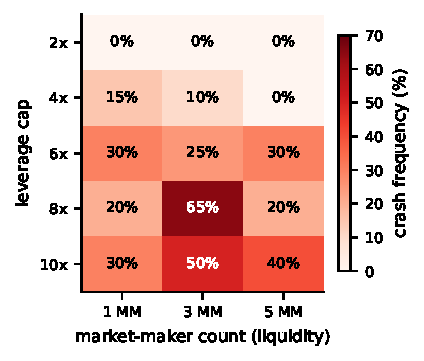
\includegraphics[width=0.8\columnwidth]{fig_levliq_heatmap.pdf}
\caption{Crash frequency across the leverage$\times$liquidity map
(300 runs, $n{=}20$ per cell, re-executed at the audited commit). The
maximum sits at $8\times$ leverage with \emph{medium} liquidity.}
\label{fig:heatmap}
\end{figure}

\begin{figure}[t]
\centering
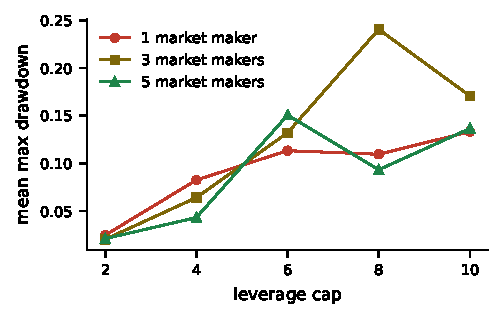
\includegraphics[width=\columnwidth]{fig_leverage_dd.pdf}
\caption{Mean maximum drawdown versus leverage cap by market-maker
count (same 300 runs).}
\label{fig:levdd}
\end{figure}

\subsection{Regime-Conditioned Strategy Example}
To illustrate the S4 bridge end to end, a flash-crash world was built
from a registered preset experiment and the EMA-crossover reference
strategy was evaluated against it (Table~\ref{tab:strategy},
Fig.~\ref{fig:regime}). The world's fingerprint records 64.3\% stable,
7.0\% crisis, and 28.8\% recovery occupancy with a detected crash;
mean fill slippage versus mid in the crisis regime ($0.100$) is
$3.4\times$ its stable-regime level ($0.029$)---the execution-cost
signature of the engineered liquidity collapse, measured by the
bridge's regime attribution rather than reconstructed after the fact.
Single world, single strategy: an illustration of the measurement
surface, not a strategy claim.

\begin{table}[t]
\caption{Strategy-evaluation example: EMA cross on a flash-crash world
(single seed; illustrative)}
\label{tab:strategy}
\centering
\scriptsize
\begin{tabular}{lr@{\qquad}lr}
\toprule
total return & $+0.096\%$ & orders / fill events & 158 / 159 \\
max drawdown & $0.064\%$ & turnover & 1.57M \\
slippage vs.\ mid (mean) & $0.029$ & & \\
\midrule
\multicolumn{4}{l}{\textbf{By regime} (PnL / fills / mean slippage)} \\
stable & \multicolumn{3}{l}{$-535.0$ / 102 / 0.029} \\
crisis & \multicolumn{3}{l}{$+540.1$ / 2 / \textbf{0.100}} \\
recovery & \multicolumn{3}{l}{$+950.0$ / 55 / 0.026} \\
\bottomrule
\end{tabular}
\end{table}

\begin{figure}[t]
\centering
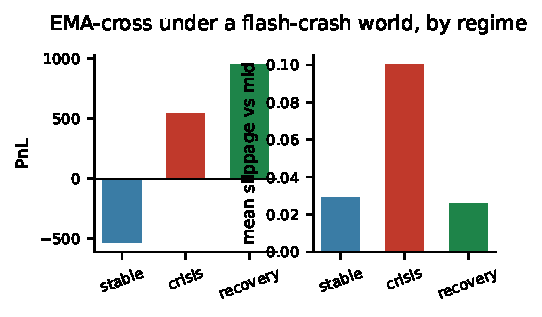
\includegraphics[width=\columnwidth]{fig_regime_strategy.pdf}
\caption{Regime-conditioned strategy metrics for the example of
Table~\ref{tab:strategy}.}
\label{fig:regime}
\end{figure}

\section{Discussion}
\label{sec:discussion}
Three observations organize the evidence. First, the platform's
scientific value materialized exactly where its design intended: the
leverage$\times$liquidity study produced a \emph{rejected}
pre-registered hypothesis and an unanticipated mechanism
(transmission-channel liquidity) that was diagnosable only because
forced liquidation is real order flow and every intermediate quantity
is artifact-backed. A system optimized for confirmation would have
reported the leverage effect and stopped. Second, reproducibility
compounds: because experiment identity is content-addressed over
configuration, schema, seed plan, and code version, specifications
committed several phases earlier re-minted identical research hashes
at the audited commit---turning ``the result still stands'' from a
claim into a checkable property. Third, the outward bridges preserve
epistemic boundaries by construction: external observations are proxies
that inform design; synthetic worlds are environments with identities;
strategies are observers with hashed configurations. Each boundary is
enforced by types, tests, and language in the artifacts themselves,
which we consider as much a contribution as any single mechanism.

\section{Limitations and Threats to Validity}
\label{sec:limits}
(1) The synthetic ecology is not a real market; all findings are
statements about a specified model. (2) Agent behavioral models are
deliberately simple; richer cognition could change dynamics
qualitatively. (3) Calibration can be non-identifiable; the platform
demonstrated this concretely (agent count), and any calibration claim
is bounded by identifiability. (4) External event-market integration
establishes observation, not causation; divergence and lead/lag
metrics are observational. (5) Prediction-market prices are
market-implied probability proxies, not ground truth
\cite{wolfers2004}. (6) No licensed real-market dataset is bundled;
stylized-fact comparisons in this paper use synthetic targets, and
real-data validation remains open. (7) The NautilusTrader bridge
treats strategies as observers; absent feedback, market-impact and
crowding questions are out of scope. (8) Synthetic worlds reproduce
selected properties, not all properties, of real markets. (9)
Reported wall-times are environment-dependent; the determinism
guarantees are not, but performance figures should not be quoted as
platform constants. (10) Several conclusions (e.g., the
transmission-channel result) are configuration-dependent: single
asset, one venue, market-order liquidation, no funding network. (11)
Causal language in this paper is strictly intra-model; higher-order
causal inference (mediation, dose-response designs) requires further
experiment types. (12) Crash detection is a drawdown threshold, not a
validated event definition---an F0-documented definitional limitation.

\section{Future Research}
\label{sec:future}
(a) Bidirectional \tez{}$\leftrightarrow$NautilusTrader co-simulation
in which a strategy becomes a participant in the ecology, gated on an
explicit synchronization contract (time authority, same-timestamp
event ordering, latency modeling, order-injection boundary, feedback
timing, checkpointing, and a coupled reproducible identity)---no
implementation before that contract is specified. (b) Richer agent
cognition (learning, heterogeneous horizons) with the same provenance
guarantees. (c) Multi-asset ecologies and cross-asset contagion,
including funding networks that would directly re-test the
transmission-channel finding. (d) Rigorous empirical calibration
against licensed real datasets, with block-bootstrap uncertainty on
the target side and ABC/history-matching methods. (e) Distributed
Monte Carlo beyond single-machine workers, and GPU acceleration only
where it preserves bit-level determinism. (f) Richer microstructure
(latency, queue position, fees, multiple venues). (g) Event-market
driven scenario generation at scale: standing pipelines from
Kalshi/Polymarket event signatures to controlled experiment proposals
under human approval. (h) Higher-$n$ replication of the $8\times$
leverage row and formal tests for the non-monotone liquidity effect.
(i) A natural-language hypothesis compiler and an AI research-analyst
layer are \emph{future work}: no LLM component exists in the current
system, and the documented policy for any future analyst confines it
to reading artifacts and proposing hypotheses behind human approval,
never entering the deterministic measurement loop. (j) Synthetic-world
benchmark suites and research-artifact publication infrastructure
(e.g., archived experiment bundles with DOIs).

\section{Conclusion}
\label{sec:conclusion}
\tez{} demonstrates that the standards of experimental science---
pre-registered designs, replication, statistical inference, immutable
identity, provenance, and reproduction---can be engineered directly
into a market-simulation platform rather than appended to it. The
platform's own flagship study behaved the way science should: a large
main effect was confirmed, a pre-registered interaction was rejected,
and an unanticipated mechanism emerged that was traceable to a specific
modeling decision (liquidation as real order flow) through
artifact-backed evidence, and the entire chain reproduces from
content-addressed identities at a later commit. The system now spans
observation (read-only event markets), synthesis (controlled market
worlds), and evaluation (strategy backtests), with one provenance
thread connecting them. \tez{} predicts nothing about real markets;
its contribution is a laboratory in which mechanism hypotheses about
markets become falsifiable, replicable, and reproducible experiments.

\section*{Reproducibility Statement}
All experiments in this paper are reproducible from the repository at
commit \texttt{af12ef0756c8} (380 passing, 7 skipped). The complete
loop is:
{\footnotesize\begin{verbatim}
tezcat run examples/leverage_liquidity_map.json
tezcat analyze expv_60fabaa6f7ca
tezcat report  expv_60fabaa6f7ca -o report.md
tezcat reproduce 60fabaa6
\end{verbatim}}
\texttt{reproduce} re-executes sampled runs and verifies seeds, state
hashes, event hashes, event-log chains, and metrics against stored
artifacts; the analogous verbs exist for market worlds
(\texttt{tezcat lab reproduce}) and full research-plane chains
(\texttt{tezcat plane reproduce}), both of which fail loudly on
dependency-version mismatch. Figures in this paper were generated by
the committed scripts in \texttt{paper/figures/}; the paper build is
one command (\texttt{paper/build.sh}). The repository README declares
an MIT license; no DOI or archived research-artifact identifier exists
at the audited commit, and none is claimed.

\balance
\bibliographystyle{IEEEtran}
\bibliography{references}

\end{document}
